\section{State of art}

% \subsection{Theorethical framework}
% \begin{frame}{Theorethical framework}
%   \begin{block}{Context}
%     In \citep{Bellavista2012} several definitions of context are listed:
%     \begin{itemize}
%       \item Context contains information addressing "where you are, who you are with, and what resources are nearby", [Schilit et al. 1994].
%       \item Context contains "any information that can be used to characterize the situation of an entity", [Dey and Abowd 2000].
%       \item Context comprises "elements for the description of this context information [that] fall into five categories: individually, activity, location, time, and relations", [Zimmermann et al. 2007].
%       \item Context is the "set of variables that may be of interest for an agent and that influence its actions", [Bolchini et al. 2009].
%       \item \textbf{Context is "a four-dimensional space composed of \emph{computing context}, \emph{physical context}, \emph{time context}, and \emph{user context}", [Chen and Kotz 2000].}
%     \end{itemize}
%   \end{block}
% \end{frame}


\subsection{Mobile sensing apps}

\begin{frame}{Mobile sensing apps (MSA)}
  \begin{block}{Definition of MSA}
    The set of mobile apps that perform tasks related to data collection from sensors and information discovery from these data.
  \end{block}

  \begin{block}{Reasons of the success of MSA}
    \begin{itemize}
      \item The increasing computing, storage, and communication capabilities existing in smart devices.
      \item The multi-modality sensing capabilities included in smart devices.
      \item The millions of smart devices already \emph{deployed} around the world.
      \item Smart devices can cover a wide and dynamic geographic area.
    \end{itemize}
  \end{block}
\end{frame}

\begin{frame}{MSA: an overview}
  \begin{block}{MSA: an overview}
  \begin{itemize}
    \item Stages of MSA operation
    \begin{itemize}
      \item \textbf{Sensor reading.}
      \item Filtering (optional).
      \item Feature extraction.
      \item Classification.
      \item Post-processing.
    \end{itemize}

    \item Sensing scale of MSA
    \begin{itemize}
      \item \textbf{Individual.}
      \item Community.
    \end{itemize}

    \item Sensing paradigms of MSA
    \begin{itemize}
      \item \textbf{Opportunistic.}
      \item Participatory.
    \end{itemize}

  \end{itemize}
  \end{block}
\end{frame}

% \begin{frame}{MSA: an overview}
%   \begin{block}{Stages of MSA}
%     \begin{figure}
%       \centering
%       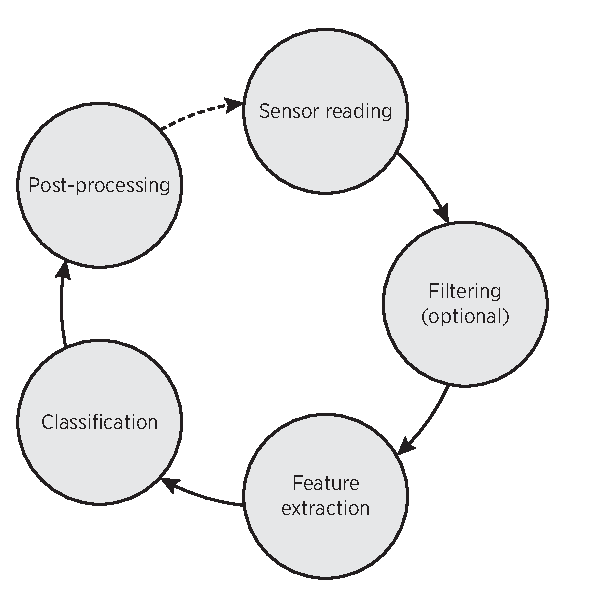
\includegraphics[scale=0.5]{msa-stages}
%       \caption[Common stages of mobile sensing apps]{Common stages of mobile sensing apps.}
%       \label{fig-mobile-sensing-apps-stages}
%     \end{figure}
%     % \begin{itemize}
%     %   \item Sensor reading.
%     %   \item Filtering (optional).
%     %   \item Feature extraction.
%     %   \item Classification.
%     %   \item Post-processing.
%     % \end{itemize}
%   \end{block}
% \end{frame}

% \begin{frame}{MSA: an overview}
%   \begin{block}{Sensing scale of MSA}
%     \begin{itemize}
%       \item Individual.
%       \item Community.
%     \end{itemize}
%   \end{block}

%   \begin{block}{Sensing paradigms of MSA}
%     \begin{itemize}
%       \item Opportunistic.
%       \item Participatory.
%     \end{itemize}
%   \end{block}
% \end{frame}

\begin{frame}{MSA: Examples}
  \begin{block}{Examples of MSA}
    \begin{itemize}
      \item \emph{NeuroPhone} \citep{Campbell2010}
      \begin{itemize}
        \item A brain-controlled address book dialing app that employs neural signals obtained from an EEG\footnote{EEG, electroencephalography} headset.
        \item The phone shows a sequence of pictures of contacts and a special signal is elicited when a photo matches the person whom the user wishes to call.
      \end{itemize}

      \item \emph{BeWell} \citep{Lane2012}
      \begin{itemize}
        \item BeWell continuously tracks user behavior along three health dimensions in an opportunistic sensing way.
        \begin{itemize}
          \item Sleep duration \rightTextArrow accelerometer.
          \item Physical activity \rightTextArrow accelerometer.
          \item Social interaction \rightTextArrow microphone.
        \end{itemize}
      \end{itemize}
  
      \item \emph{WalkSafe} \citep{Wang2012}
      \begin{itemize}
        \item An app that aids people that walk and talk, improving the safety of pedestrian phone users.
        \item WalkSafe employs the back camera of the mobile phone to detect vehicles approaching the user, alerting a potentially unsafe situation.
      \end{itemize}
    \end{itemize}
  \end{block}
\end{frame}

% \begin{frame}{Convergence of MSA into the Internet of Things}
%   \begin{block}{Convergence of MSA into the Internet of Things}
%     \begin{itemize}
%       \item MSA are contributing to the adoption of smart devices by society.
%       \item This will produce a world where people are globally connected with others.
%       \item The idea has been also pursued in scenarios like industry, where the items to be connected are real world objects like tools, machines, etc.
%       \item The items are enhanced with identification mechanisms and storage, computing and communication facilities, becoming \emph{smart objects}.
%     \end{itemize}
%   \end{block}
% \end{frame}

% \begin{frame}{Convergence of MSA into the Internet of Things}
%   \begin{block}{Convergence of MSA into the Internet of Things}
%     \begin{itemize}
%       \item The interaction of smart objects creates a Machine-to-Machine (M2M) communication system.
%       \item M2M communication systems aim to be the base mechanism to interconnect any smart objects of the real world.
%       \item MSA and M2M communication systems are pursuing a globally connected world of people and smart objects.
%       \item They can be abstracted as systems that interconnect \emph{things} in an evolved version of Internet called the \emph{Internet of Things (IoT)}.
%       \item IoT aims to produce a fully connected world with application systems that address any real world problem.
%     \end{itemize}
%   \end{block}
% \end{frame}

\subsection{Energy issues in MSA}
\begin{frame}{Energy issues in MSA}
  \begin{block}{Energy issue in MSA }
    \begin{itemize}
      \item Actual fact: The usage of components of smart devices implies energy consumption.
      \item Several efforts have been done in the field to address the issue.
      
      They can be categorized as:
      \begin{itemize}
        \item General guidelines.
        \item Focused on sensors' usage.
      \end{itemize}
    \end{itemize}
  \end{block}
\end{frame}

\begin{frame}{Energy issues in MSA: General guidelines}
  \begin{block}{General guidelines}
    \begin{itemize}
      \item Authors in \citep{Mayo2004} introduced the idea of the \emph{requirements-aware energy scale-down} approach.
      \item It states that energy consumption should be reduced as possible and still achieving mobile app requirements.
    \end{itemize}
  \end{block}

  \begin{figure}
      \centering
      \subfloat[Original interface\label{fig:energy-aware-gui-1}]{
        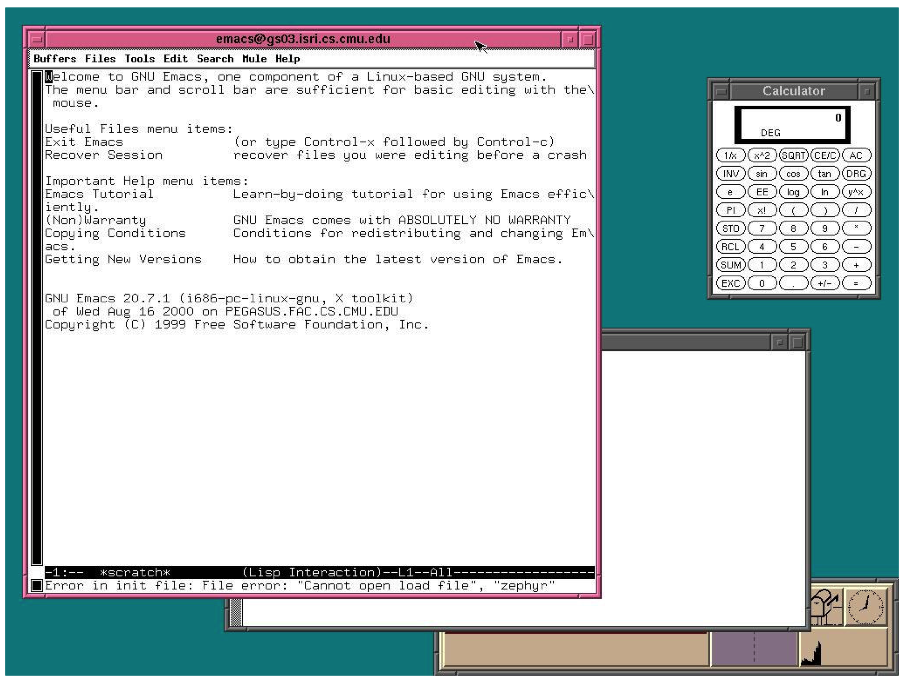
\includegraphics[width=0.3\textwidth]{energy-aware-gui-1}
      }%\quad
      \subfloat[Background half dim\label{fig:energy-aware-gui-2}]{
        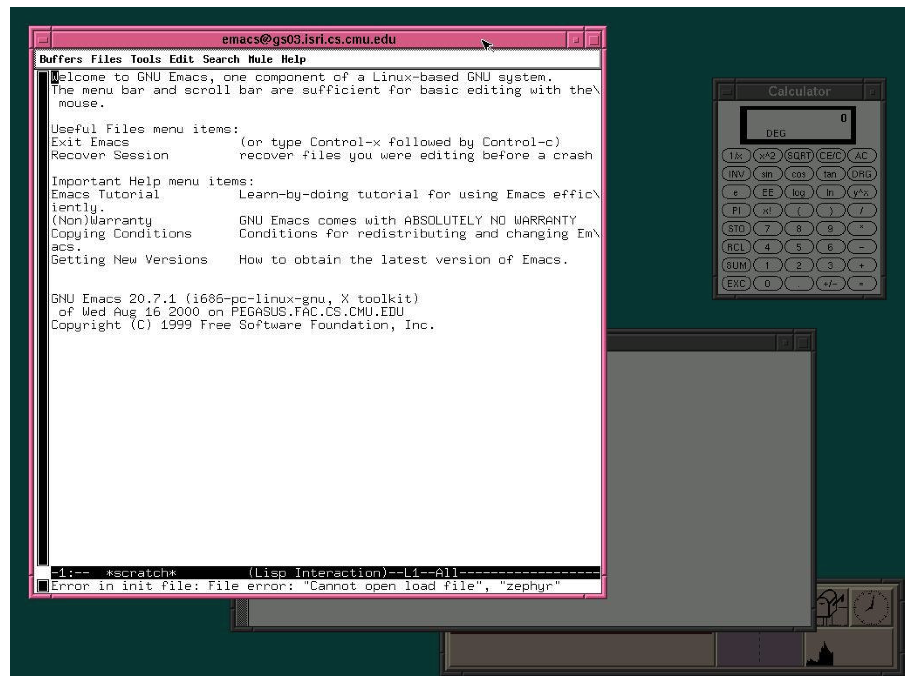
\includegraphics[width=0.3\textwidth]{energy-aware-gui-2}
      }%\quad
      \subfloat[Background fully dim\label{fig:energy-aware-gui-3}]{
        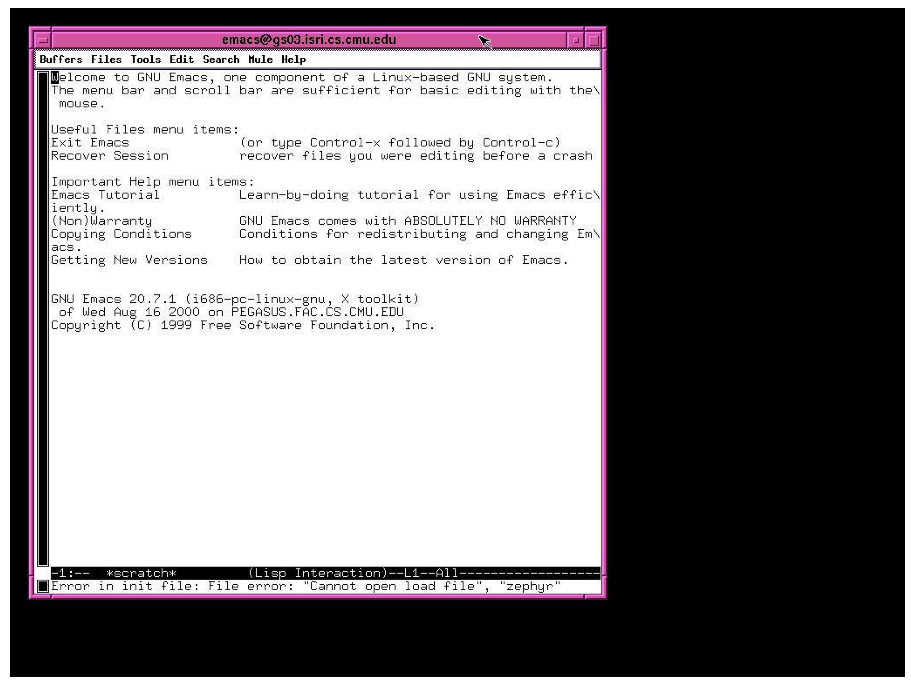
\includegraphics[width=0.3\textwidth]{energy-aware-gui-3}
      }
      \caption{An example of energy aware GUI proposed by \protect\citep{Mayo2004}}
      \label{fig-scaling-down-screen-usage}
    \end{figure}
\end{frame}

\begin{frame}{Energy issues in MSA: Efforts focused in sensors' usage}
\footnotesize
  \begin{columns}
      \column{0.5\textwidth}
        % \centering
        \begin{figure}
        \begin{tikzpicture}[thick,scale=0.23, every node/.style={scale=0.55}]
          
          % \tikzset{level 1 concept/.append style={sibling angle=90,level distance = 9mm}}
          \tikzset{every child/.append style={level distance=100mm}} 
          % \path[mindmap,concept color=hsrmWarmGreyLight,text=hsrmWarmGreyDark]
          \path[mindmap,concept color=hsrmSec1Dark,text=white]
          node[concept] {Approaches}
          [clockwise from=-30]
          child[concept color=hsrmSec1,text=white] { node[concept] {\textcolor{white}{Pure-hardware}} }
          child[concept color=hsrmSec1CompDark,text=white] { node[concept] {Hardware-Software} }
          child[concept color=hsrmSec1Comp,text=white] { node[concept] {\textcolor{white}{Pure-software}} };
        \end{tikzpicture}
        \caption{Approaches for solving the energy issue.}
        \end{figure}
      
      \column{0.5\textwidth}
        \begin{figure}
          \centering
          %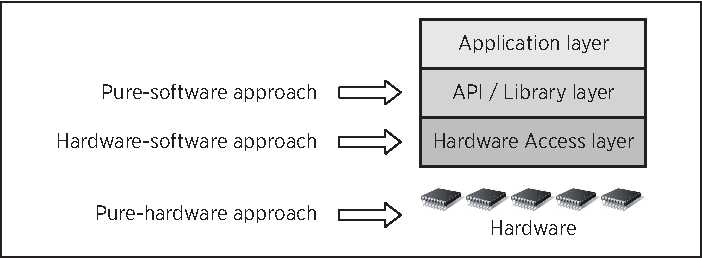
\includegraphics[scale=0.4]{cross-layer-approaches}
          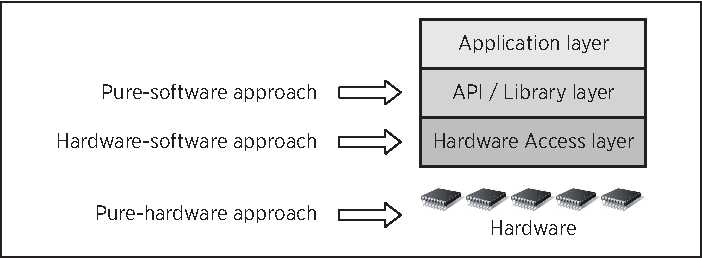
\includegraphics[width=\textwidth]{cross-layer-approaches}
          \caption{ The relation between approaches for solving the energy issue and layers of a mobile platform.}
          \label{fig-cross-layer-approaches}
        \end{figure}
        
      \end{columns}
  % % \begin{block}{Sensors' usage}
  %   \centering
  %   \begin{tikzpicture}[scale=0.78]
  %     %\tikzset{every child/.append style={level distance=250}} 
  %     % \path[mindmap,concept color=hsrmWarmGreyLight,text=hsrmWarmGreyDark]
  %     \path[mindmap,concept color=hsrmSec1Dark,text=white]
  %     node[concept] {Approaches}
  %     [clockwise from=-30]
  %     child[concept color=hsrmSec1,text=white] { node[concept] {\textcolor{white}{Pure-hardware}} }
  %     child[concept color=hsrmSec1CompDark,text=white] { node[concept] {Hardware-Software} }
  %     child[concept color=hsrmSec1Comp,text=white] { node[concept] {\textcolor{white}{Pure-software}} };
  %   \end{tikzpicture}
  % % \end{block}
\end{frame}

% \begin{frame}{Energy issues in MSA: Efforts focused in sensors' usage}
%   \begin{block}{Energy issue as a cross layer problem}
%     \begin{figure}
%       \centering
%       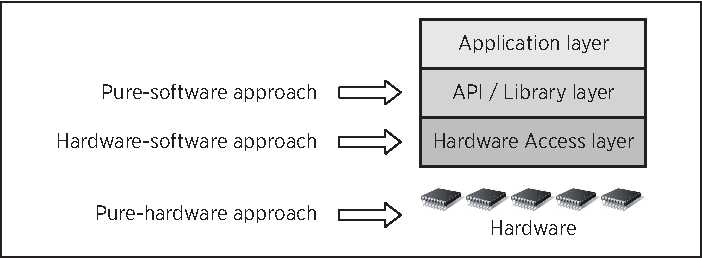
\includegraphics[scale=0.6]{cross-layer-approaches}
%       \caption[Energy issue as an OS cross-platform problem]{The relation between approaches for solving the energy issue and layers of a mobile platform.}
%       \label{fig-cross-layer-approaches}
%     \end{figure}
%   \end{block}
% \end{frame}

\begin{frame}{Energy issues in MSA: Efforts focused in sensors' usage}
  \begin{block}{Pure-hardware approach}
    \begin{itemize}
      \item Electronic level techniques like DPM\footnote{Dynamic Power Management.} or DVFS\footnote{Dynamic Voltage and Frequency Scaling.} are not enough to mark the energy issue as solved \citep{Priyantha2011}.
      \item Current architecture of mobile platforms requires that for the correct operation of the phone other components have to be operational
      \item This approach aims to redesign the hardware platform of current mobile devices, by isolating sensors inside a unit with a dedicated low power processor.
      \item While the extra unit is working the rest of the smartphone hardware platform can reach its sleep mode.
    \end{itemize}
  \end{block}
\end{frame}

\begin{frame}{Energy issues in MSA: Efforts focused in sensors' usage}
  \begin{block}{Examples of works following a pure-hardware approach}
    \begin{itemize}
      \item LittleRock \citep{Priyantha2011} designs a special unit in charge of the execution of sensor readings.
      It includes:
      \begin{itemize}
        \item Processor module.
        \item Digital sensor module.
        \item Analog sensor module.
        \item Reset and wake up logic.
      \end{itemize}

      \item \citep{Choudhury2008} implemented a mobile sensing platform with embedded sensors and a low power processor.
      Includes also bluetooth communication interface.
    \end{itemize}
  \end{block}
\end{frame}

\begin{frame}{Energy issues in MSA: Efforts focused in sensors' usage}
  \begin{block}{Hardware-software approach}
    \begin{itemize}
      \item This approach aims to contribute with new drivers, tunned versions of mobile OS's or an improved software API for allocating computational and sensing tasks in components others than the predefined by the platform's original design.
      \item It is possible to instruct an additional low power processor in the smartphone to execute any arbitrary instruction.
      \item Since the smartphone's processor can be kept idle there is a potential energy saving.
    \end{itemize}
  \end{block}
\end{frame}

\begin{frame}{Energy issues in MSA: Efforts focused in sensors' usage}
  \begin{block}{Examples of works following a hardware-software approach}
  \begin{itemize}
    \item The study presented by \citep{Ra2012} leverages the presence of low power processors (LP) in the latest smartphones, exposing their functionality through a layered API.

    \item It describes two challenges:
    \begin{enumerate}
       \item The selection of a suitable LP: any processor with a small wakeup transition delay is suitable as LP.
       \item Guidelines for deciding where to allocate the execution of a given task:
       \begin{itemize}
          \item Execution in main processor.
          \item Execution in LP.
          \item Execution in main or in LP.
      \end{itemize}
    \end{enumerate}
  \end{itemize}
  \end{block}
\end{frame}

\begin{frame}{Energy issues in MSA: Efforts focused in sensors' usage}
  \begin{block}{Pure-software approach}
  \begin{itemize}
    \item The goal of this approach is to give \emph{smartness} or cognitive behavior to the software platform of mobile devices and derive into a better usage of sensors.
    \item Two main branches (not mutually exclusive):
    \begin{itemize}
      \item Duty cycle manipulation
      \item Next value inference
    \end{itemize}
  \end{itemize}
  \end{block}
\end{frame}

\begin{frame}{Energy issues in MSA: Efforts focused in sensors' usage}
  \begin{block}{Examples of works following a pure-software approach}
  \begin{itemize}
    \item \emph{G-Sense} \citep{Perez2010}
    \begin{itemize}
      \item An architecture that integrates mobile and static WSN for location based services, participatory sensing and human centric sensing applications.
      \item Include mechanisms to control the amount of generated and transmitted data: \emph{client-sate machine}, \emph{Geo-Sensing}, and \emph{Time-Sensing}.
      \item It was not implemented, only simulated.
      \item Its mechanisms are a very broad genre of policies.
    \end{itemize}
    \item EnTracked \citep{Kjaergaard2009}
    \begin{itemize}
      \item Platform to perform GPS readings in smartphones; employs also accelerometer to detect motion.
      \item Employs a external server to detect the speed of user; scenarios without Internet connectivity are ignored.
      \item Involve costs in data transmission.
    \end{itemize}
  \end{itemize}
  \end{block}
\end{frame}

\begin{frame}{Energy issues in MSA: Efforts focused in sensors' usage}
  \begin{block}{Examples of works following a pure-software approach}
    Middleware in \citep{Perez-Torres2012}.
    \begin{itemize}
      \item A power-aware middleware for context aware mobile apps with cloud computing interaction focused on GPS data.
      \item Allows to schedule the next sensor reading according to the mobile app specifications and other policies.
      \item Includes rudimentary notions of policies, classifier and mobile app specific requirements.
    \end{itemize}
  \end{block}
\end{frame}

\begin{frame}{Energy issues in MSA: Efforts focused in sensors' usage}
  \begin{block}{Advantages of pure-software approach}
    \begin{itemize}   
      \item
        Modifying hardware and/or updating the mobile OS\footnote{OS, Operating System.} of existing devices is almost impossible.
      \item
        Implementations of pure-hardware and hardware-software approaches are application specific.
      \item
        A pure-software approach can be implemented in a software unit and embedded in a mobile app as any other 3rd party library.
      \item
        Cognitive processes can be conducted directly in a high software layer and re-configured and tunned.
      \item 
        A pure-software approach is not mutually exclusive with pure-hardware and hardware-software approaches.
    \end{itemize}
  \end{block}
\end{frame}

\subsection{Energy issue in data transmission}

\begin{frame}{Energy issue in data transmission}
  \begin{block}{Data transmission effects in energy consumption}
    \begin{itemize}
      \item The energy consumption also represents a problem when transmitting data or performing computation offloading.
      \item This perspective of the problem has also been addressed in literature and several solutions have been provided.
      \item Computation offloading is advisable only when large amount of computations are needed with relatively small amounts of communication \citep{Kumar2010}.
      \item The transmission of data can be guided by the presence of changes in the data collected by sensors \citep{Musolesi2010}.
      \item In relation to MSA, this issue becomes critical when the mobile apps focus in the community sensing scale.
    \end{itemize}
  \end{block}
\end{frame}

% \begin{frame}{Energy issue in data transmission}
%   \begin{block}{Computation offloading from ECI perspective}
%   \begin{itemize}
%     \item In \citep{Kumar2010} a basic decision-making strategy to determine whether computation offloading should be done is presented.
%   \end{itemize}
%     \begin{figure}
%       \centering
%       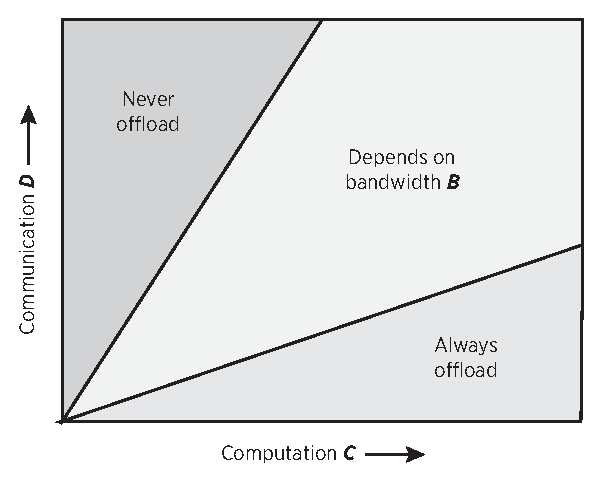
\includegraphics[scale=0.5]{offloading-decision-chart}
%       \caption[Computational offloading decision strategy]{Computation offloading decision chart.}
%       \label{fig:offloading-decision-chart}
%     \end{figure}
%   \end{block}
% \end{frame}

% \begin{frame}{Energy issue in data transmission}
%   \begin{block}{Computation offloading from MD perspective}
%     \begin{itemize}
%       \item On-line strategies
%       \begin{itemize}
%         \item Always upload.
%         \item Upload in presence of changes.
%         \item Upload in presence of persistent changes.
%         \item Voting based upload strategy.
%       \end{itemize}
%       \item Off-line strategies
%       \begin{itemize}
%         \item Involves uncertainty.
%         \item They are based on the probability of change from a state into another.
%         \item The data is not sent but predicted at back-end.
%       \end{itemize}
%       \item Intermittent network connectivity
%       \begin{itemize}
%         \item Useful when network connectivity is intermittent and it is not possible to predict data.
%         \item Employ a store and forward protocol.
%         \item For instance, CarTel \citep{Hull2006} defines a network stack for a delay tolerant communication.
%       \end{itemize}
%     \end{itemize}
%   \end{block}
% \end{frame}

\begin{frame}{Scope of research}
  \begin{exampleblock}{Scope of research}
    The mechanisms to be produced:
    \begin{itemize}
      \item will follow a \emph{pure-software approach} for the creation of mobile sensing apps;
      \item will collect data at an \emph{individual sensing scale}, and
      \item will access sensors in an \emph{opportunistic paradigm} over long periods of time in a continuous way.
    \end{itemize}

    The analysis, design, and generation of policies will be implemented focusing in the usage of the GPS receiver and mobility data.
  \end{exampleblock}
\end{frame}